\documentclass{beamer}
\usetheme{default}
\usepackage[ngerman]{babel}
\usepackage[utf8x]{inputenc}
\usepackage{pgf}

\title{Softwareprojekt 2 Abschlusspräsentation}
\subtitle{Gruppe WOYM}
\date{08.02.2015}
\author{Tim Hansen\\ Adrian Lück\\ Jurij Schmidt}
\institute{Universität Bremen}
\titlegraphic{
\includegraphics[width=2cm,height=2cm]{../WOYM.png}}
\setbeamertemplate{footline}[text line]{%
  \parbox{\linewidth}{\vspace*{-8pt}\hfill\insertshortauthor\hfill\insertpagenumber}}
\setbeamertemplate{navigation symbols}{}
\begin{document}
\maketitle

\section{Projektverlauf}
\begin{frame}
\frametitle{Gliederung}
\tableofcontents[currentsection]
\end{frame}

\begin{frame}
\frametitle{Zeitplan}
\begin{itemize}
\item geplanter Aufwand entsprach relativ genau dem tatsächlichen Aufwand
\item Zeitplan für Implementierung wurde lediglich um ca. 10 Tage verlängert
\end{itemize}
\end{frame}

\begin{frame}
\frametitle{Probleme}
\begin{itemize}
\item Drei Gruppenmitglieder haben sich nicht am Projekt beteiltigt.\\ \vspace{10pt}
	{\usebeamercolor[fg]{structure} Umgang mit dem Problem:} Trennung von diesen Mitgliedern
\end{itemize}
\end{frame}

\begin{frame}
\frametitle{Probleme}
\begin{itemize}	
\item Problem mit inkonsistenten Rückgabewerten von bestimmten Datenbankanfragen\\ \vspace{10pt}
	{\usebeamercolor[fg]{structure} Umgang mit dem Problem:} Workaround durch andere Anfragen oder auf Java-Ebene
\end{itemize}
\end{frame}

\begin{frame}
\frametitle{Probleme}
\begin{itemize}	
\item Problem mit dem Zwischenspeicher der Datenbank durch falsche Verwendung der erhaltenen Objekte\\ \vspace{10pt}
{\usebeamercolor[fg]{structure} Umgang mit dem Problem:} Anpassung der Verwendung der Objekte
\end{itemize}
\end{frame}


\section{Statistiken}

\begin{frame}
\frametitle{Gliederung}
\tableofcontents[currentsection]
\end{frame}

\begin{frame}
\frametitle{Commits nach Jahr}
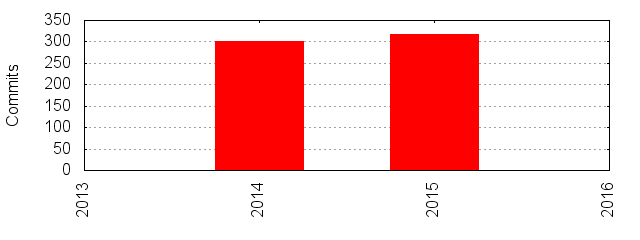
\includegraphics[width=\textwidth]{images/commits_by_year.png}
\end{frame}

\begin{frame}
\frametitle{Commits nach Wochentagen}
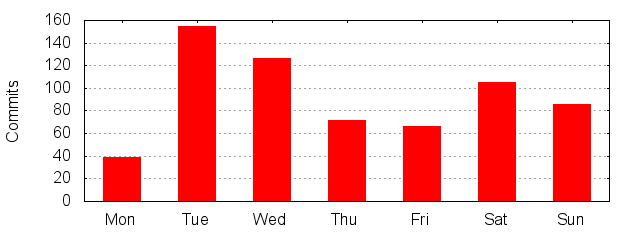
\includegraphics[width=\textwidth]{images/day_of_week.png}
\end{frame}

\begin{frame}
\frametitle{Commits nach Uhrzeit}
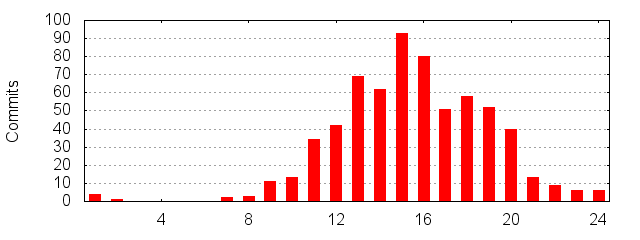
\includegraphics[width=\textwidth]{images/hour_of_day.png}
\end{frame}

\begin{frame}
\frametitle{Aktivität nach Wochen}
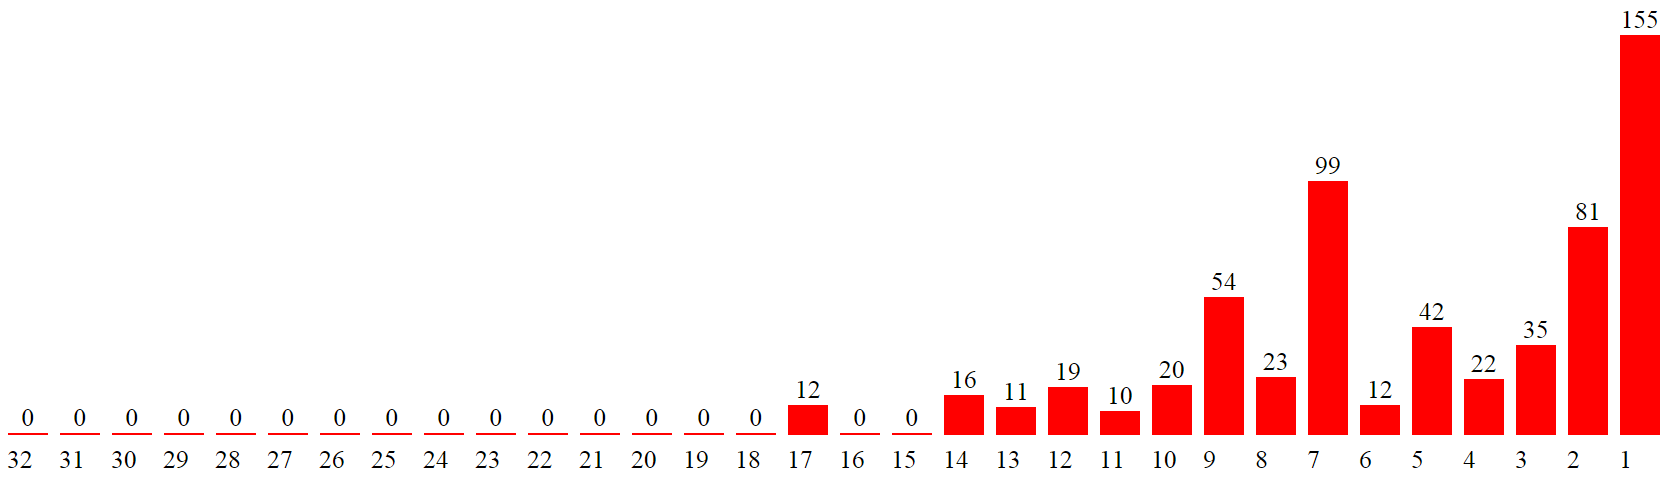
\includegraphics[width=\textwidth]{images/weekly_activity.png}
\end{frame}

\begin{frame} 
  \frametitle{Lines of Code}
  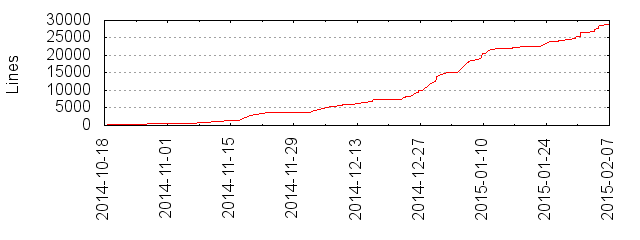
\includegraphics[width=\textwidth]{images/lines_of_code.png}
\end{frame}

\begin{frame}
\frametitle{Lines of Code nach Dateitypen}
\renewcommand{\arraystretch}{2}
\begin{table}
\centering
\begin{tabular}{ccc}
Java: & 24.755 & 84,89 \%\\
XHTML: & 3.670  & 12,58 \%\\
Sonstige: & 718  & 2,53 \%\\
\hline\hline
Insgesamt: & 29143 & 100 \%\\
\end{tabular}
\end{table}
\end{frame}

\section{Fazit}
\begin{frame}
\frametitle{Gliederung}
\tableofcontents[currentsection]
\end{frame}

\begin{frame}
\frametitle{Was nehmen wir mit?}
\begin{itemize}
\item neue Kenntnisse in JavaServer Faces / Primefaces
\item neue Kenntnisse mit der Java Persistence API (JPA)
\item neue Kenntnisse über Kollaborationsmöglichkeiten (z.B. Waffle)
\item verbesserte Git-Kenntnisse
\item eine Projekterfahrung
\end{itemize}
\end{frame}

\begin{frame}

\section{Fragen?}
\begin{center}

\Large
Vielen Dank für Ihre Aufmerksamkeit. \\\hspace{20pt}

\huge
{\usebeamercolor[fg]{structure} Fragen?}
\end{center}
\end{frame}

\end{document}